\documentclass[a4paper,12pt]{report}
\usepackage{natbib}
\usepackage{subcaption}
\usepackage{cleveref}
\usepackage{packages/rapportutc}
\usepackage[nottoc, notlof, notlot]{tocbibind}
\usepackage{sidecap}
\usepackage{array}
\usepackage[linewidth=1pt]{mdframed}


\usepackage{packages/Sweave} %package d'affichage des codes R
\usepackage{amsmath, amsthm, amssymb, graphics, setspace} %packages de mathématiques
\usepackage{calc,enumitem}  % Mise en forme l'environnement itemsize description etc.
%\usepackage{subfigure, wrapfig} % pour avoir plusieurs figures alignées  
\usepackage{color}
\usepackage{ae,aecompl}
\usepackage{pifont}
\usepackage{chemist} %formule chimique 
\usepackage{comment}
\usepackage{rotating}
\usepackage{hyperref}
\usepackage{listings}



%\usepackage{biblatex}

%%%%%%%%%%%%%%%%%%%%%%%%%%%%%%%%%%%%%%%%%%%%%%%%%%%%%%%%%%%%%%%%%%%%%%%%%%%% 

\title{TP 1 - Statistique descriptive, Analyse en composantes principales}
\author{LU Han - HAMONNAIS Raphaël}
\date{\today}

\uv{SY09}
\branche{Génie Informatique}
\filiere{Fouille de Données et Décisionnel}
%%%%%%%%%%%%%%%%%%%%%%%%%%%%%%%%%%%%%%%%%%%%%%%%%%%%%%%%%%%%%%%%%%%%%%%%%%%%

\begin{document}
\renewcommand{\labelitemi}{\large\textcolor{tatoebagreen}{\fg}}
\newgeometry{top=2.5cm,bottom=2cm,left=2cm,right=2cm}
\groovypdtitre
\restoregeometry % restaure la géométrie par défaut de latex

%%%%%%%%%%%%%%%%%%%%%%%%%%%%%%%%%%%%%%%%%%%%%%%%%%%%%%%%%%%%%%%%%%%%%%%%%%%% 

\tableofcontents

%%%%%%%%%%%%%%%%%%%%%%%%%%%%%%%%%%%%%%%%%%%%%%%%%%%%%%%%%%%%%%%%%%%%%%%%%%%%



\chapter{Statistique descriptive}

\section{Notes de SY02 au semestre de printemps 2016}

\subsection{Analyse descriptive}

\paragraph{Description des données}


Le jeu de données contient des informations relatives aux 296 étudiants inscrits à l’UV SY02 au semestre de printemps 2016 ainsi que les résultats qu'ils ont obtenus. On a donc 296 mesures (individus de la population) représentés par onze variables~: 8 qualitatives et 3 quantitatives.\\
Liste des variables qualitatives~:
\begin{itemize}
	\item \textbf{nom} : nom de l'étudiant, au format texte (nons anonymisés, au format "Etu1, Etu2,~...").
	\item \textbf{specialite} : spécialité de l'étudiant, $\in$ \{GB, GI, GM, GP, GSM, GSU, HuTech, ISS, TC\}.
	\item \textbf{niveau} : le numéro du semestre actuel de l'étudiant, $ \in \{1,2,3,4,5,6\} $.
	\item \textbf{statut} : vaut $ \{UTC,Echange\} $ selon que c'est un étudiant de l'UTC ou bien un étudiant originaire d'une autre université effectuant une partie de ses études à l'UTC.
	\item \textbf{dernier.diplome.obtenu} : le dernier diplôme obtenu par l'étudiant, $\in$ \{AUTRE 1ER CYCLE, AUTRE 2E CYCLE AUTRE DIPLOME SUPERIEUR, BAC, BTS, CPGE, DEUG, DUT, ETRANGER SECONDAIRE, ETRANGER SUPERIEUR, INGENIEUR, LICENCE, NA's\}.
	\item \textbf{correcteur.median} et \textbf{correcteur.final} : le correcteur ayant corrigé la copie (nons anonymisés au format "Cor 1,~...").
	\item \textbf{resultat} Le résultat de l'étudiant, de \textit{A} à \textit{F} ou \textit{ABS} s'il a été absent à l'un des deux examens (final ou médian). \textit{F} et \textit{Fx} signifient que l'étudiant n'a pas obtenu l'UV, les autres notes qu'il l'a obtenue.
\end{itemize}
Liste des variables quantitatives~:
\begin{itemize}
	\item \textbf{note.median} : la note obtenue au médian ($ \in [0;20] $).
	\item \textbf{note.final} : la note obtenue au final ($ \in [0;20] $).
	\item \textbf{note.totale} : la moyenne des deux notes, pondérée par l'importance de chaque note.
\end{itemize}


\paragraph{Données manquantes}
On remarque qu'il manque certaines informations dans les données (R le spécifie avec le mot clé "\textit{NA's}" pour \textit{Not Available} en anglais).
\begin{itemize}
	\item Correcteur du médian et/ou du final~: élève absent au médian et/ou au final.
	\item Dernier diplôme obtenu~: donnée manquante pour les étudiants en échange.
	\item Note au médian et/ou au final~: donnée manquante pour les étudiants absents ou qui ont abandonné.
	\item Résultat~: donnée "manquante" pour R qui considère la valeur \textit{ABS} comme étant manquant car \textit{resultat} est une variable qualitative ordonnée et \textit{ABS} ne fait pas partie des différents niveau d'ordre. Représente donc des élèves absents qui n'ont pas obtenu l'UV.
\end{itemize}


\paragraph{Intuitions statistiques~: liens supposés entre les variables}
De manière logique, on pourrait penser que les notes entre le médian et le final sont liées, un élève bon au médian étant plus à même de réussir le final et inversement. De même, la formation d'origine de l'étudiant devrait fortement influencer l'obtention de l'UV. Un étudiant venant de tronc commun (diplôme d'origine BAC) a logiquement plus de change de réussir qu'un élève venant de DUT. Le correcteur ne devrait logiquement pas influencer les notes, la notion d'équité entre les copies étant très importante.




\subsection{Etude des liens statistique entre les variables}

\paragraph{Pré-requis}
On considère que les données ont été préalablement nettoyées en enlevant tous les étudiants absents, c'est à dire qui n'ont pas eu l'UV pour cause d'absence accidentelle ou d'abandon pur et simple.

\paragraph{Procédure}

Nous utiliserons le test d'indépendance du $\chi^2$ qui permet de vérifier l'indépendance de deux variables X et Y : 

\begin{itemize}
	\item Hypothèse nulle $H_{0}$~: les deux variables X et Y sont indépendantes.
	\item Hypothèse $H_{1}$~: les deux variables X et Y ne sont pas indépendantes.
	\item On rejette l'hypothèse nulle lorsque \textit{p-value} est inférieure ou égale à 0,05. La valeur \textit{p-value} représente la probabilité d'obtenir la même valeur (ou une valeur encore plus extrême) du test si l'hypothèse nulle était vraie.
	\item Toutes les cases du tableau de contingence doivent avoir une valeur supérieure ou égale à 5. Le tableau de contingence est un tableau à double entrée représentant les effectifs partiels des observations en fonction des variables X en ligne et Y en colonne.
\end{itemize}



\subsubsection{Lien statistique entre le résultat et le diplôme d'origine des étudiants}
La première étape fut de nettoyer les données en supprimant les 6 étudiants dont le statut vaut \textit{Echange} car leur diplôme d'origine n'est pas renseigné.\\
Nous avons ensuite créé le tableau de contingence, qui donne pour chaque valeur de la variable \textit{resultat} le nombre d'élèves ayant obtenu ce résultat en fonction de leur diplôme d'origine~: on obtient un effectif pour chaque couple \textit{diplôme d'origine}/\textit{résultat}.

\begin{figure}[h]
	\centering
	\captionsetup{justification=centering, margin=2cm}
	\begin{subfigure}[b]{0.5\linewidth}
		\centering
		\captionsetup{justification=centering, margin=1cm}
		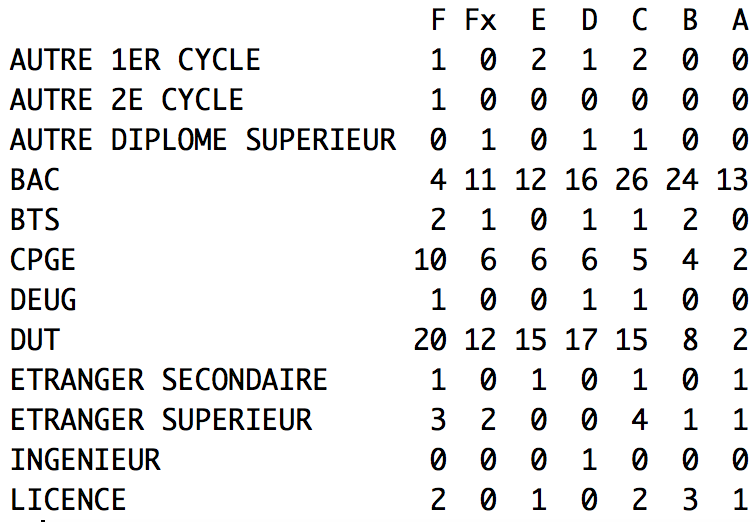
\includegraphics[width=0.65\linewidth]{img/1-1-2-Contingence-Result-Diplome-Origine}
		\caption{\scriptsize Tableau de contingence entre résultats et diplôme d'origine}
		\label{fig:tab_contingence_diplome_resultat}
	\end{subfigure}%
	\begin{subfigure}[b]{0.5\linewidth}
		\centering
		\captionsetup{justification=centering, margin=1cm}
		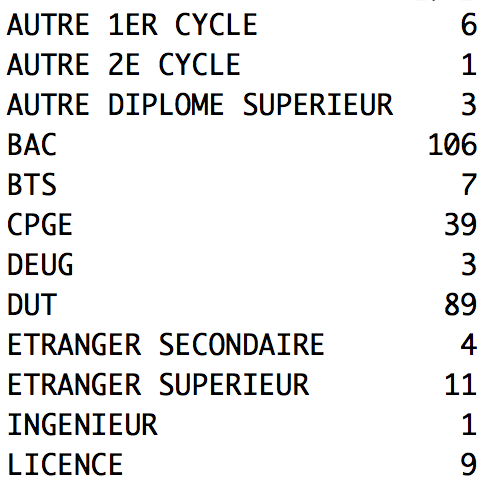
\includegraphics[width=0.5\linewidth]{img/1-1-2-Effectif-Diplome-Origine}
		\caption{\scriptsize Effectif total par diplôme}
		\label{fig:effectif_total_par_diplome}
	\end{subfigure}%
	\caption{
		\small Effectifs de la population par diplôme d'origine et tableau de contingence entre les variables \textit{résultat} et \textit{diplôme d'origine}.
	}
	\label{fig:tab_effectifs_et_contingence_resultats_diplome_origine}%
\end{figure}

On remarque immédiatement que les conditions du test ne sont pas respectées~: il a y une majorité des effectifs qui sont inférieurs à 5 dans le tableau de contingence  (cf. figure \ref{fig:tab_contingence_diplome_resultat}). Et c'est tout à fait normal si l'on regarde les effectifs d'étudiants (figure \ref{fig:effectif_total_par_diplome}) en fonction de leur diplôme d'origine dans la population totale~: seuls les diplômes BAC (étudiant venant de tronc commun), DUT et CPGE sont convenablement représentés.
On peut tout de même effectuer le test du $\chi^2$ tout en sachant que les conditions ne sont pas respectées, afin de vérifier l'importance de ces conditions. On obtient alors une \textit{p-value} égale à $0.2572$. On conserve donc l'hypothèse $H_{0}$ d'indépendance des variables, tout en sachant que le résultat et probablement faux.

\paragraph{Correction des effectifs}
Afin de respecter les conditions du test de $\chi^2$, nous n'avons gardé que les lignes correspondant aux diplômes d'origines de type \textit{BAC}, \textit{DUT} et \textit{CPGE}. Il a aussi fallut regrouper les deux premières et deux dernières classes de \textit{résultat} en sommant les effectifs des élèves ayant obtenu \textit{F} ou \textit{Fx} et ceux ayant eu \textit{A} ou \textit{B}.\\
On obtient ainsi un nouveau tableau de contingence~:

\begin{figure}[h]
	\centering
	\captionsetup{justification=centering, margin=2cm}
	\begin{subfigure}[b]{0.5\linewidth}
		\centering
		\captionsetup{justification=centering, margin=1cm}
		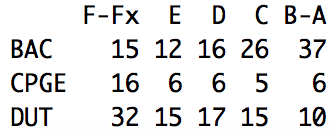
\includegraphics[width=0.5\linewidth]{img/1-1-2-Contingence-Result-Diplome-Corrigee}
		\caption{\scriptsize Tableau de contingence \textbf{corrigé} entre les variables \textit{résultat} et \textit{diplôme d'origine}.}
		\label{fig:tab_effectifs_et_contingence_resultats_diplome_origine_corrigee}
	\end{subfigure}%
	\begin{subfigure}[b]{0.5\linewidth}
		\centering
		\captionsetup{justification=centering, margin=1cm}
		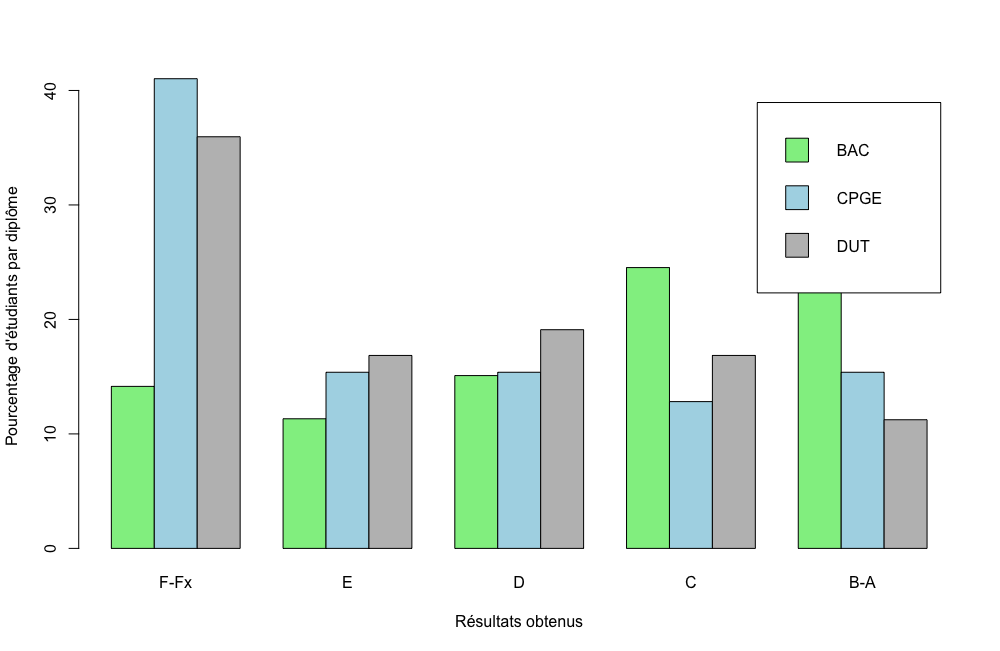
\includegraphics[width=1\linewidth]{img/1-1-2-Ratio-resultat-diplome}
		\caption{\scriptsize Effectif total par diplôme}
		\label{fig:ratio_resultats_diplome}
	\end{subfigure}%
	\caption{
		\small Tableau de contingence \textbf{corrigé} et visualisation des fréquences entre les variables \textit{résultat} et \textit{diplôme d'origine}.
	}
	\label{fig:tab_frequence_et_contingence_corriges_resultats_diplome_origine}%
\end{figure}
Les conditions du test sont alors réunies et on obtient une \textit{p-value} égale à $0.000288$. On rejette donc l'hypothèse $H_{0}$ d'indépendance avec confiance~: le diplôme d'origine d'un étudiant a un impact significatif sur son résultat final à l'UV de statistiques SY02. On voit bien sur le graphique en barre représentant les fréquence d'obtention d'un résultat en fonction du diplôme d'origine (cf. figure \ref{fig:ratio_resultats_diplome}) qu'un peu plus de 15\% des élèves ayant comme dernier diplôme le BAC ont obtenu \textit{A} ou \textit{B} tandis que seulement 2\% d'entre-eux n'ont pas réussi l'UV. On remarque aussi que la courbe est croissante~: plus le résultat est bon, plus la fréquence d'obtention augmente. Pour les élèves provenant de DUT ou CPGE par contre c'est l'inverse~: moins le résultat est bon, plus la fréquence augmente.


\subsubsection{Lien statistique entre le résultat et la spécialité des étudiants}



\subsubsection{Lien statistique entre le résultat et la niveau des étudiants}



\subsubsection{Lien statistique entre le résultat et les correcteurs}




\section{Données Crabs}


\end{document}